%-------------------------------------------------------
% Comandos para os algoritmos:
\renewcommand{\algorithmicfor}{\textbf{para}}
\renewcommand{\algorithmicif}{\textbf{se}}
\renewcommand{\algorithmicthen}{\textbf{então}}
\renewcommand{\algorithmicelse}{\textbf{senão}}
\renewcommand{\algorithmicendif}{\textbf{fim se}}
\renewcommand{\algorithmicendfor}{\textbf{fim para}}
\renewcommand{\algorithmicdo}{\textbf{faça}}
%-------------------------------------------------------

\chapter{Desenvolvimento do modelo OLAP}
\label{cap:DesenvolvimentoDoModeloOLAP}
%-------------------------------------------------------
% descrever como foi feito o levantamento dos residuos mais interesantes. 
%  Explicar que a lista dos mais presentes foi comparada com uma lista originalmente desenvolvida por um especialista de dominio. 
%  Encontrou se casos que estavam e nao estavam na lista, os que nao apareciam na lista constituem de residuos que se ficam ˜proximos”ao sitio de ligação, mas que na realidade estão fora do sítio.
% descrever como  adicionar novas dimensoes baseadas em novos residuos
%-------------------------------------------------------
\section{Levantamento de questões de negócio}
\label{sec:LevantamentoDeQuestoesDeNegocio}

Para possibilitar a construção do modelo OLAP, primeiramente foi necessário identificar e definir as questões de negócio que seriam relevantes sob o ponto de vista do especialista de domínio. Em virtude disso, o levantamento destes dados foi feito por meio de entrevistas com os especialistas do LABIO.

A Tabela \ref{tab:questaoNegocio} descreve as questões de negócio que foram identificadas como sendo mais relevantes para execução de análise de experimentos de docagem realizados no LABIO. 

\begin{table}[h]
\caption{Questões de negócio identificadas pelos especialistas com maior relevância para análise de experimentos de docagem}
\label{tab:questaoNegocio}
\centering
\resizebox{\textwidth}{!}{%
\begin{tabular}{@{}ll@{}}
\toprule
\textbf{ } & \multicolumn{1}{c}{\textbf{Questões de maior relevância para a análise de docagem}}		\\ \midrule
\textbf{1.} & Associar um grupo para cada conformação;													\\
\textbf{2.} & Identificar o comportamento das conformações baseado nas métricas de FEB e RMSD;			\\
\textbf{3.} & Identificar conformações/grupos que possuem o maior número de contatos com os ligantes;	\\
\textbf{4.} & Com base no item 3, identificar quais são os resíduos mais importantes;					\\
\textbf{5.} & Com base no item 3, identificar quais grupos possuem melhores valores de FEB e RMSD.		\\ \bottomrule
\end{tabular}
}
\end{table}

\section{Identificação de métricas}
\label{sec:IdentificacaoDeMetricas}

Durante as entrevistas realizadas, pode-se perceber que informações baseadas nas métricas FEB e RMSD possuíam grande relevância para responder as questões de negócio. Entretanto foi necessário definir certas propriedades e limitações de valores para adequar os cálculos às necessidades do negócio. Dessa maneira, todas as definições citadas nesta seção foram estabelecidas em conjunto com os especialistas de domínio do LABIO, para que os resultados apresentados pudessem representar a realidade.

O cálculo da FEB é um dos métodos utilizados pelos softwares de docagem que permite avaliar a interação receptor-ligante. Quanto menor for o resultado deste cálculo, mais favorável é a ligação estabelecida. Portanto, o valor estimado da FEB é utilizado como uma das métricas do modelo.

Na maioria dos experimentos, os melhores resultados de FEB são valores negativos. Portanto, qualquer conformação que apresente valores de FEB positivos não foram levados em consideração. Dessa maneira evita-se que os resultados positivos venham a interferir em uma análise futura dos valores agregados de um experimento. 

O cálculo do RMSD é utilizado para obter a distância média entre os átomos. Nos experimentos de docagem, este cálculo é feito para comparar o posicionamento inicial do ligante, geralmente estipulada pelo especialista de domínio, com o posicionamento final após a execução da docagem. Neste caso, o RMSD é considerado como uma métrica para a modelagem.

Tanto a FEB quando o RMSD dão uma visão para o especialista de quão satisfatório foi o processo de docagem para uma determinada iteração. Enquanto a FEB mede a qualidade da docagem no aspecto termodinâmico da questão, o RMSD tem como natureza avaliar geometricamente como estão dispostas as moléculas do resíduo e do ligante.

Além disso, para ser possível responder ao item 3 da Tabela \ref{tab:questaoNegocio}, foi necessário incluir uma métrica para contabilizar o número de contatos entre o ligante e um resíduo da molécula receptora. 

Um contato pode ser identificado pelo cálculo da medida em {\AA}ngstr\"om ({\AA}) entre os átomos do resíduo do receptor e do ligante. Ou seja, para cada resíduo do receptor \emph{R} é calculada a distância Euclidiana entre todos seus átomos e os átomos de um ligante \emph{L}. Sendo $R=(r_{x},r_{y},r_{z})$ representando as coordenadas dos átomos dos resíduos do receptor, e $L=(l_{x},l_{y},l_{z})$ representando as coordenadas dos átomos do ligante, o cálculo da distância se dá pela equação \ref{eqt:distEuclid}.

\begin{equation}
\label{eqt:distEuclid}
	d(R,L)=\sqrt{(r_{x}-l_{x})^{2}+(r_{y}-l_{y})^{2}+(r_{z}-l_{z})^{2}}
\end{equation}

Em suma, para cada snapshot devem ser calculadas todas as coordenadas do receptor com todas as coordenadas de cada ligante, neste caso para o TCL e para o ETH. Entretanto, de todas as distâncias calculadas para um resíduo, apenas a menor delas deve ser considerada. 

A Figura \ref{fig:PIFvsGLY} ilustra este conceito, apresentando como exemplo as distâncias entre os átomos do ligante PIF (cor preto) e do resíduo GLY95 (cor cinza) do receptor InhA. Para todas as distâncias calculadas, a menor delas é de 2.72 {\AA} \cite{KARANADUNOSM09}.

\begin{figure}[h]
	\center
	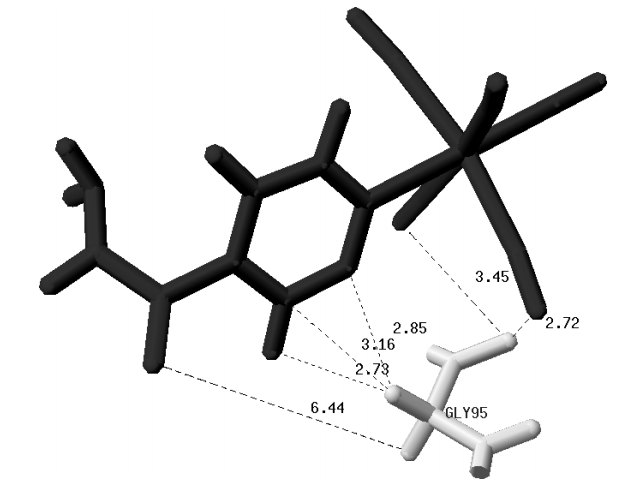
\includegraphics[scale=0.55]{images/distEucli.png}
	\caption{Cálculo das distâncias atômicas entre o ligante PIF (cor preta) e o resíduo GLY95 (cor cinza) do receptor InhA \cite{KARANADUNOSM09}.}
	\label{fig:PIFvsGLY}
\end{figure} 

\section{Definição de relevância para os resíduos}

Um dos pontos mais importantes para responder aos questionamentos dos especialistas de domínio e fundamental para composição das dimensões, consiste em definir os resíduos que são mais relevantes para os experimentos de docagem envolvendo os ligantes TCL e ETH com o receptor InhA. 

A enzima InhA é composta por 268 resíduos, e o processo de identificação dos mais importantes leva em consideração o número de contatos estabelecidos entre os átomos do resíduo e o ligante. No \emph{data set} que foi resultado do processo de simulação de docagem, cada átomo do resíduo está representado por uma tripla, contendo a sua localização espacial nos eixos \emph{x, y }e \emph{z}.

De acordo com o especialista de domínio, a interação entre um átomo do resíduo e o ligante só deve ser considerada como contato quando a distância entre ambos seja entre 2{\AA} e 4{\AA}. Valores inferiores a 2{\AA} são descartados por serem considerados uma sobreposição, enquanto valores superiores a 4{\AA} indicam que não foi estabelecido contato. 

Além disso, uma outra restrição se aplica para os átomos de hidrogênio dos resíduos da molécula receptora. Por apresentarem um comportamento diferente, os átomos de hidrogênio são desconsiderados e não têm suas distâncias calculadas.

Dessa forma, para cada resíduo do receptor deve ser calculada a distância Euclidiana tridimensional de seus átomos utilizando a equação \ref{eqt:distEuclid}, conforme descrito na seção \ref{sec:IdentificacaoDeMetricas}. A partir daí, identifica-se a relevância de um resíduo para o experimento de docagem conforme o número de contatos que são estabelecidos entre seus átomos e o ligante. Quanto mais contatos, mais relevante o resíduo é para o experimento.

As regras de classificação de relevância de um resíduo podem ser sumarizadas da seguinte forma:
\begin{itemize}
	\item Considerar como contatos somente as distâncias entre 2 e 4 {\AA}ngstr\"ons.
	\item Desconsiderar distâncias inferiores a 2 {\AA}ngstr\"ons.
	\item Desconsiderar átomos de hidrogênio.
	\item Quanto maior for o número de contatos estabelecidos de um resíduo, mais relevante ele se torna para o experimento.
\end{itemize}

Assim que foram definidas as limitações e regras de classificação, o esforço foi aplicado na obtenção destes dados. 

Com base em estudos e análises de experimentos anteriores utilizando a InhA como molécula receptora, um especialista de domínio elaborou uma lista dos 52 principais resíduos que possuem relevância para os experimentos de docagem baseados no mesmo cenário. Este artefato foi levado em consideração e serviu como base para identificar os resíduos que fossem relevantes. 

A Tabela \ref{tab:listaOsmar} apresenta a lista elaborada pelo especialista contendo os resíduos representados pela sua sigla e seu número de ordem na enzima.

\begin{table}[h]
\caption{Lista elaborada pelo especialista de domínio com os principais resíduos para experimentos de docagem utilizando a enzima InhA.}
\label{tab:listaOsmar}
\centering
\begin{tabular}{@{}lllllll@{}}
GLY\_13	&	PHE\_40 &	PHE\_96	&	PHE\_148 &	PRO\_191 &	ILE\_201 &	GLU\_209 		\\
ILE\_14	&	LEU\_62 &	MET\_97	&	PRO\_155 &	ILE\_193 &	VAL\_202 &	ALA\_210 		\\
ILE\_15	&	ASP\_63 &	GLN\_99	&	ALA\_156 &	THR\_195 &	GLY\_203 &	ILE\_214 		\\
THR\_16	&	VAL\_64 &	MET\_102 &	TYR\_157 &	LEU\_196 &	GLY\_204 &	LEU\_217 		\\
SER\_18	&	GLN\_65 &	GLY\_103 &	MET\_160 &	ALA\_197 &	ALA\_205 &					\\
SER\_19	&	SER\_93 &	ILE\_121 &	LYS\_164 &	MET\_198 &	LEU\_206 &					\\
ILE\_20	&	ILE\_94	&	MET\_146 &	ALA\_190 &	SER\_199 &	GLY\_207 &					\\
ALA\_21 &	GLY\_95	&	ASP\_147 &	GLY\_191 &	ALA\_200 &	GLU\_208 &					\\ 
\end{tabular}
\end{table}

\section{Identificação dos resíduos relevantes}
\label{sec:IdentificacaoDosResiduosRelevantes}

Durante a fase de desenvolvimento dos scripts necessários para processamento dos dados de docagem e extração das informações relevantes, foi identificada a necessidade de dividir o \emph{data set}. De acordo com os especialistas de domínio, o resíduo NAH deveria ter sua distância euclidiana calculada apenas com o ligante TCL.

Como no \emph{data set} original todas as informações estavam consolidadas em um único arquivo CSV contendo 3.100 linhas e 12.335 colunas, a manipulação destes dados em softwares como o Microsoft Excel se torna praticamente inviável.

Dessa forma, foi desenvolvido um \emph{script} nomeado de ``ajustaColunasDocking'' para fazer a manipulação das colunas do \emph{data set}. O script recebe os seguintes parâmetros de entrada:

\begin{enumerate}
	\item Sinal da operação a ser feita (`-m' mantém as colunas, e `-e' remove as colunas);
	\item Nome das colunas que serão manipuladas separadas por vírgula;
	\item Arquivo de entrada com dados de docagem (\emph{data set});
	\item Arquivo de saída com as colunas manipuladas.
\end{enumerate}

O Algoritmo \ref{alg:ajustaColunaDocking} descreve o processo de funcionamento do script ``ajustaColunasDocking''.

\floatname{algorithm}{Algoritmo}
\begin{algorithm}[H]
\caption{Algoritmo para manipulação da base de dados da simulação de docagem molecular}
\label{alg:ajustaColunaDocking}
{\fontsize{10}{10}\selectfont
\begin{algorithmic}[1]
	\STATE Seja C a lista com o nome das colunas
	\STATE Seja D a base de dados dos resultados da simulação de docagem molecular
	\STATE Seja c uma coluna em C
	\STATE Seja d uma linha em D
	\STATE Seja M o modo de operação da execução
	\IF{M for igual a manter as colunas em C}
		\FOR{cada d em D}
			\FOR{cada c em C}
			\STATE Grave apenas c na saída
			\ENDFOR
		\ENDFOR
	\ENDIF
	\IF{M for igual a excluir as colunas em C}
		\FOR{cada d em D}
			\FOR{cada c em C}
			\STATE Remove apenas c na saída
			\ENDFOR
		\ENDFOR
	\ENDIF
\end{algorithmic}
}
\end{algorithm}

O algoritmo ``ajustaColunasDocking'' foi utilizado para remover os dados referentes aos átomos do resíduo NAH do \emph{data set} original e separá-los em outro arquivo de dados distinto. Após a manipulação, os arquivos de dados ficaram da seguinte forma:
\begin{itemize}
	\item \emph{Data set} 1: Removidas todas as colunas dos átomos referentes ao resíduo NAH.
	\item \emph{Data set} 2: Apenas dados dos átomos referentes ao resíduo NAH e do ligante TCL.
\end{itemize}

Neste ponto é importante ressaltar que ambos os arquivos tiveram somente suas colunas alteradas e mantiveram um total de 3.100 linhas, representando a trajetória das conformações da molécula receptora.

Com os arquivos devidamente separados de acordo com os critérios estabelecidos, foi possível realizar o cálculo da distância Euclidiana. Para isso, foi desenvolvido um segundo script, nomeado ``calculaDistancia'', que realiza o cálculo de todo o conjunto de átomos existente em um \emph{data set} tendo como base os critérios definidos previamente para classificação da relevância dos resíduos.

Para execução do script ``calculaDistancia'', são necessários três parâmetros de entrada, sendo eles:
\begin{enumerate}
	\item Arquivo contendo lista de átomos do resíduo da molécula;
	\item Arquivo contendo lista de átomos do(s) ligante(s);
	\item Arquivo de entrada com dados de docagem (\emph{data set}).
\end{enumerate}

%-----------------------------------
% 
%    TO DO: verificar as informações de saída do script
%
%       
%-----------------------------------

A partir dos três arquivos de entrada é gerado um arquivo de saída em formato CSV contendo as seguintes informações: número do snapshot, nome do resíduo, nome do ligante, resultado do cálculo da distância, classificação da distância (se foi menor que 2 ou está entre 2 e 4 {\AA}ngstr\"ons).
O Algoritmo \ref{alg:CalculoDistancia} descreve o processo de funcionamento do script "calculaDistancia.

\floatname{algorithm}{Algoritmo}
\begin{algorithm}[H]
\caption{Algoritmo para cálculo da distância}
\label{alg:CalculoDistancia}
{\fontsize{10}{10}\selectfont
\begin{algorithmic}[1]
	\STATE Seja R uma lista de resíduos
	\STATE Seja L uma lista de ligantes
	\STATE Seja D a base de dados dos resultados da simulação de docagem molecular
	\STATE Seja r um resíduo de R
	\STATE Seja l um ligante de L
	\STATE Seja d um \emph{snapshot} da conformação da base D
	\FOR{cada d em D}
		\FOR{cada r em R}
			\FOR{cada l em L faça}
			\IF{r não conter átomo de hidrogênio}
			\STATE Distância $\gets \sqrt{(rx - lx)^{2} +(ry - ly)^{2} + (rz - lz)^{2}}$ 
			\ENDIF
			\IF{Distância menor que 4}
				\IF{Distância menor ou igual a 2}
				\STATE Gravar na saída d, r, l, distancia, classificação menor que 2
				\ELSE
				\STATE Gravar na saída d, r, l, distancia, classificação entre 2 e 4
				\ENDIF
			\ENDIF
			\ENDFOR
		\ENDFOR
	\ENDFOR
\end{algorithmic}
}
\end{algorithm}

%-----------------------------------
% 
%    TO DO: colocar screenshot do output do script
%
%       
%-----------------------------------

Após a execução do algoritmo para calcular as distâncias os dados de saída foram sumarizados. Como resultado, foi obtida uma listagem de 15 resíduos com maior número de contatos comuns para os experimentos de docagem envolvendo ambos ligantes TCL e ETH. A Tabela \ref{tab:listaProvavelRelevantes} lista os resíduos obtidos pelo algoritmo, que estão representados pela sua sigla e seu número de ordem na enzima.

\begin{table}[h]
	\caption{Resíduos identificados pelo algoritmo de cálculo.}
	\label{tab:listaProvavelRelevantes}
	\centering
	\begin{tabular}{@{}lll@{}}
	ILE\_15  & ASP\_149 & MET\_160 \\
	SER\_19  & ARG\_152 & ILE\_193 \\
	ILE\_94  & ALA\_153 & THR\_195 \\
	GLY\_95  & MET\_154 & MET\_198 \\
	PHE\_148 & TYR\_157 & TRP\_221 \\
	\end{tabular}
\end{table}

Com posse destes dados, os resíduos resultantes (apresentados na Tabela \ref{tab:listaProvavelRelevantes}) foram comparados com a lista feita pelo especialista de domínio (apresentados na Tabela \ref{tab:listaOsmar}) a fim de identificar os elementos que eram comuns aos dois grupos. 

Dos 15 resíduos identificados pelo algoritmo, 10 deles estão presentes na lista do especialista de domínio e foram classificados como sendo relevantes para os experimentos de docagem. Os 5 resíduos que não estavam presentes na lista do especialista foram identificados como casos onde a proteína apresentou ligações fora da cavidade do substrato e, por este motivo, não foram considerados como sendo relevantes. Os resíduos do conjunto obtido foram plotados pelos especialistas de domínio do LABIO e estão ilustrados pela Figura \ref{fig:PlotResiduos}. 

\begin{figure}[h]
        \center
        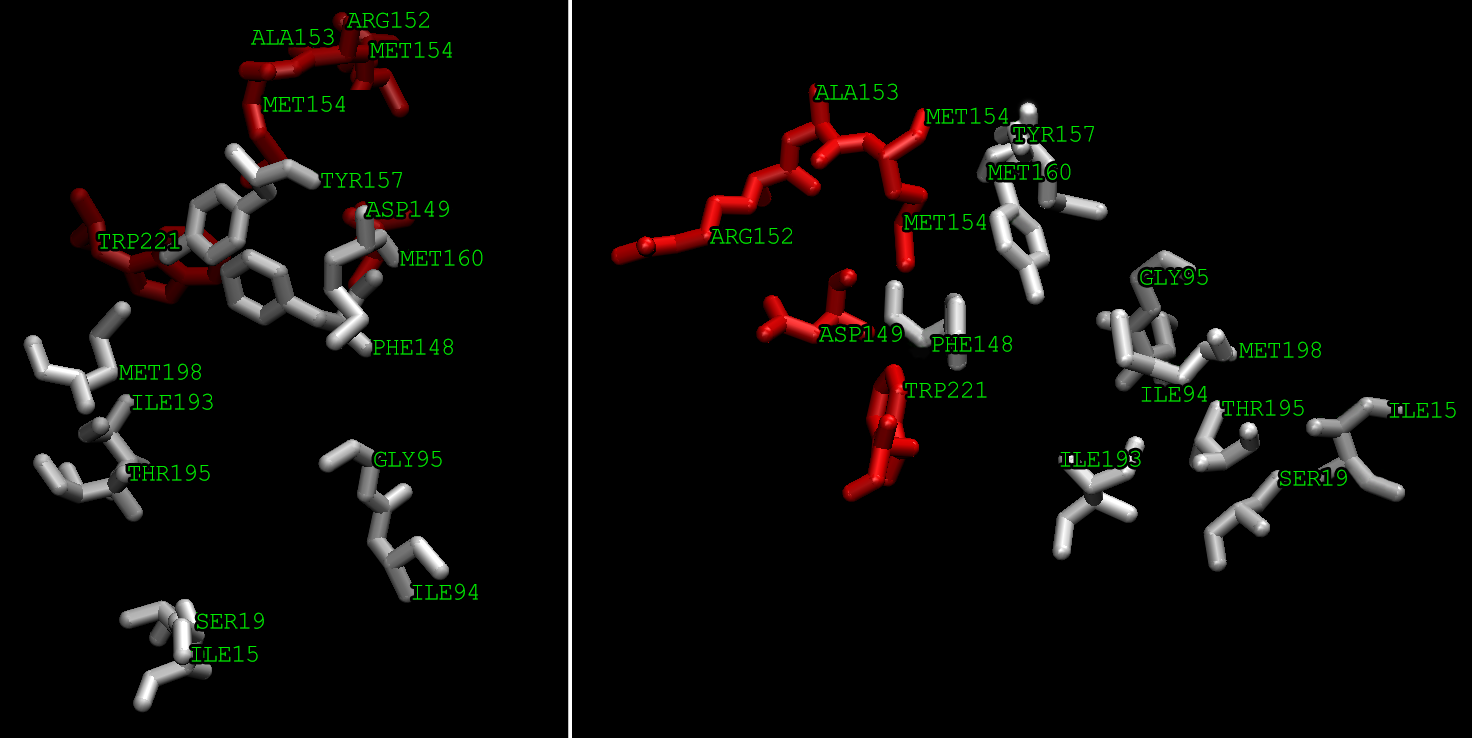
\includegraphics[scale=0.55]{images/avaliacao_Residuos_nomes.png}
        \label{fig:PlotResiduos}
        \caption{Plotagem dos 15 resíduos identificados pelo algoritmo de classificação por relevância. A cor cinza representa os resíduos que são relevantes e aparecem na listagem do especialista de domínio, já os resíduos que estão em vermelho não estão presentes na lista.}
\end{figure}

Com base nos algoritmos executados e nas comparações realizadas, foi possível elencar os 10 principais resíduos mais relevantes para responder às questões de negócio. O conjunto final está listado na Tabela \ref{tab:listaProvavelRelevantes}, a qual foi utilizada como base para a modelagem OLAP.

\begin{table}[h]
\caption{Conjunto final de resíduos relevantes para experimentos de docagem molecular considerando como receptor a enzima da InhA e ligantes TCL e ETH.}
\label{tab:listaProvavelRelevantes}
\centering
\begin{tabular}{@{}ll@{}}
\toprule
\textbf{Resíduo} 		    & \textbf{Nome} 		 \\ \midrule
SER\_19                     & Serina                   \\
ILE\_15                     & Isoleucina               \\
ILE\_94                     & Isoleucina               \\
GLY\_95                     & Glicina                  \\
PHE\_148                    & Fenilalanina             \\
TYR\_157                    & Tirosina                 \\
MET\_160                    & Metionina                \\
ILE\_193                    & Isoleucina               \\
THR\_195                    & Treonina                 \\
MET\_198                    & Metionina                \\ \bottomrule
\end{tabular}
\end{table}

\section{Modelagem da solução}
\label{sec:ModelagemDaSolucao}

Para atender às questões de negócio levantadas pelos especialistas de domínio conforme descrito na Tabela \ref{tab:questaoNegocio}, foi proposto um modelo de dados do tipo estrela contendo uma tabela fato e quinze dimensões. 

A modelagem proposta foi baseada na resolução das questões de negócio específicas para o cenário descrito neste trabalho, porém este mesmo modelo pode ser empregado em outros tipos de experimentos. A Figura \ref{fig:ConcepcaoModeloOLAP} ilustra o projeto inicial da modelagem OLAP.

\begin{figure}[h]
        \center
        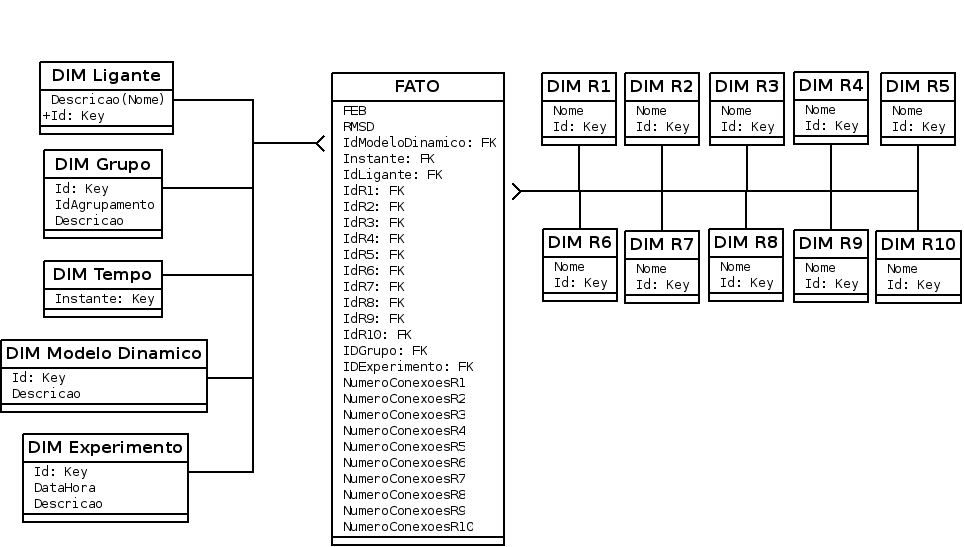
\includegraphics[scale=0.45]{images/Modelo_OLAP.png}
        \caption{Concepção inicial do modelo OLAP}
        \label{fig:ConcepcaoModeloOLAP}
\end{figure}

A tabela fato foi projetada tendo como base as métricas identificadas na Seção \ref{sec:IdentificacaoDeMetricas}, ou seja: FEB, RMSD e número de contatos. As métricas de FEB e RMSD foram representadas na tabela fato pelos atributos ``FEBMedio'' e ``RMSDMedio'', ambos utilizando o cálculo de valor médio.

Como foi elencado um conjunto contendo 10 resíduos mais importantes para o experimento, a métrica de número de contatos deve valer para cada um dos resíduos, apresentando o número de ligações entre o resíduo e o ligante. Para representar isso na fato, foram criadas as métricas \emph{``NumeroConexoesR1'', ``NumeroConexoesR2'', ..., ``NumeroConexoesR10''}, estes realizando apenas o cálculo de somatório. Já as dimensões para os resíduos, foram representadas por ``DIM\_R1'' até ``DIM\_R10''.

A dimensão ``DIM\_Ligante'' representa os ligantes utilizados no experimento, neste caso o TCL e ETH.

O conjunto de conformações utilizado é de 3.100 conformações, a qual representa a trajetória dinâmica da molecula durante 3.100 picosegundos (ps). Neste cas o número da conformação se equivale ao instante de tempo, por exemplo, o snapshot 500 refere-se a conformação da molécula receptorna no instante de 500ps. Com isso, o tempo foi representado pela dimensão ``DIM\_Tempo''. 

A dimensão ``DIM\_Modelo\_Dinamico'' serve para o especialista de domínio identificar qual foi a dinâmica utilizada no experimento. No caso deste trabalho, foi utilizada apenas uma dinâmica de 3.100 conformações.

Um experimento de docagem utiliza agrupamentos para determinadas conformações, com base na semelhança existente entre elas. Dessa forma, foi necessário permitir a que estes agrupamentos fossem identificados, para possibilitar a análise por agrupamento. Esta necessidade foi representada pela dimensão ``DIM\_Grupo''.

Por fim, a dimensão ``DIM\_Experimento'' serve para o especialista de domínio identificar as informações relacionadas ao experimento executado. Um mesmo experimento de docagem poder ser executado mais de uma vez utilizando modelos dinâmicos diferentes. Com esta dimensão os experimentos são separados com base nas informações providas pelo especialista de domínio.


\section{Construção do modelo no Analisys Services}

A modelagem inicial do OLAP se mostrou apto para responder as questões de negócio que foram levantadas no início do projeto. Com isso, modelo foi construído utilizando as ferramentas Microsoft Analysys Services e o banco de dados Microsoft SQL Server. A Figura \ref{fig:ModeloOLAP} ilustra o modelo já criado no Analysis Services.

\begin{figure}[h]
        \center
        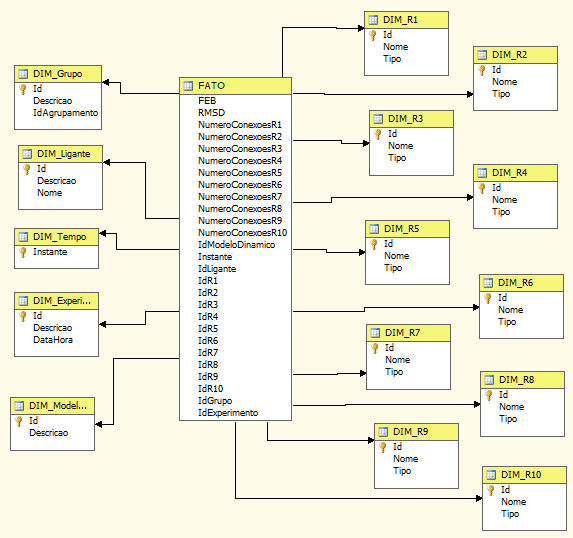
\includegraphics[scale=1]{images/ModelagemOLAP.PNG}
        \caption{Modelo OLAP construído com uso do Microsoft Analysis Services.}
        \label{fig:ModeloOLAP}
\end{figure}

A seguir descrevem-se todas as definições e propriedades levadas em consideração durante a criação do modelo OLAP no Analysis Services, bem como a definição de cada campo:
	
\begin{itemize}
	\item
		\textbf{Tabela:} DIM\_Grupo \\
		\textbf{Tipo:} Dimensional. \\
		\textbf{Descrição:} Representa os agrupamentos de conformações por semelhança.
\end{itemize}
\begin{table}[h]
	\caption{Dimensão DIM\_Grupo}
	\centering
	\begin{tabular}{@{}llll@{}}
	\toprule
	\textbf{Nome} & \textbf{Tipo} & \textbf{PK} & \textbf{Descrição}           		\\ \midrule
	Id            & INT           & x           & Identificador da dimensão grupo   \\
	Descricao     & TEXT       &             & Descrição do grupo           		\\
	IdAgrupamento & INT           &             & Identificador do agrupamento 		\\ \bottomrule
	\end{tabular}
\end{table}

% \begin{figure}[h]
%         \center
%         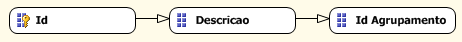
\includegraphics[scale=1]{images/A_DIM_Grupo.PNG}
%         \caption{Hierarquia da dimensão DIM\_Grupo}
%         \label{fig:ModeloOLAP}
% \end{figure}

\newpage

\begin{itemize}
	\item
		\textbf{Tabela:} Fato \\
		\textbf{Tipo:} Fato. \\
		\textbf{Descrição:} Representa todos os eventos de um experimento.
\end{itemize}
\begin{table}[!htbp]
	\caption{Tabela Fato}
	\centering
	\begin{tabular}{@{}llll@{}}
	\toprule
	\textbf{Nome} & \textbf{Tipo} & \textbf{FK} & \textbf{Descrição}           				\\ \midrule
	FEB            			 & INT        &             & Valor médio de FEB			    \\
	RMSD    				 & INT        &             & Valor médio de RMSD          		\\
	NumeroConexoesR1 	     & INT        &             & Numero de ligações do resíduo 1   \\
	NumeroConexoesR2 	     & INT        &             & Numero de ligações do resíduo 2   \\
	NumeroConexoesR3 	     & INT        &             & Numero de ligações do resíduo 3   \\
	NumeroConexoesR4 	     & INT        &             & Numero de ligações do resíduo 4   \\
	NumeroConexoesR5 	     & INT        &             & Numero de ligações do resíduo 5   \\
	NumeroConexoesR6 	     & INT        &             & Numero de ligações do resíduo 6   \\
	NumeroConexoesR7 	     & INT        &             & Numero de ligações do resíduo 7   \\
	NumeroConexoesR8 	     & INT        &             & Numero de ligações do resíduo 8   \\
	NumeroConexoesR9 	     & INT        &             & Numero de ligações do resíduo 9   \\
	NumeroConexoesR10 	     & INT        &             & Numero de ligações do resíduo 10  \\
	Instante 	    		 & INT        &  x          & Identificador do instante de tempo  \\
	IdLigante 	    		 & INT        &  x          & Identificador do Ligante 			\\
	IdR1 				     & INT        &  x          & Identificador do resíduo 1   	\\
	IdR2 				     & INT        &  x          & Identificador do resíduo 2   	\\
	IdR3 				     & INT        &  x          & Identificador do resíduo 3   	\\
	IdR4 				     & INT        &  x          & Identificador do resíduo 4   	\\
	IdR5 				     & INT        &  x          & Identificador do resíduo 5   	\\
	IdR6 				     & INT        &  x          & Identificador do resíduo 6   	\\
	IdR7 				     & INT        &  x          & Identificador do resíduo 7   	\\
	IdR8 				     & INT        &  x          & Identificador do resíduo 8   	\\
	IdR9 				     & INT        &  x          & Identificador do resíduo 9   	\\
	IdR10			 	     & INT        &  x          & Identificador do resíduo 10  	\\	
	IdGrupo			 	     & INT        &  x          & Identificador do grupo  		\\	
	IdExperimento 			 & INT        &  x          & Identificador do experimento 	\\ \bottomrule
	\end{tabular}
\end{table}

\begin{itemize}
	\item
		\textbf{Tabela:} DIM\_Tempo \\
		\textbf{Tipo:} Dimensional. \\
		\textbf{Descrição:} Representa o tempo em picosegundo. \\
\end{itemize}
\begin{table}[h]
	\caption{Dimensão DIM\_Tempo}
	\centering
	\begin{tabular}{@{}llll@{}}
	\toprule
	\textbf{Nome} 	& \textbf{Tipo} & \textbf{PK} & \textbf{Descrição}           		\\ \midrule			
	Instante 		& INT 	       &  x           & Instante de tempo 					\\ \bottomrule
	\end{tabular}
\end{table}

\begin{itemize}
	\item
		\textbf{Tabela:} DIM\_Ligante \\
		\textbf{Tipo:} Dimensional. \\
		\textbf{Descrição:} Representa o ligante utilizado no experimento. \\
\end{itemize}
\begin{table}[h]
	\caption{Dimensão DIM\_Ligante}
	\centering
	\begin{tabular}{@{}llll@{}}
	\toprule
	\textbf{Nome} & \textbf{Tipo} & \textbf{PK} & \textbf{Descrição}           		   \\ \midrule
	Id            & INT           & x           & Identificador da dimensão ligante    \\
	Descricao     & TEXT       &             & Descrição do ligante           	   \\
	Nome 		  & TEXT       &             & Nome do ligante 					   \\ \bottomrule
	\end{tabular}
\end{table}

% \begin{figure}[h]
%         \center
%         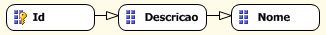
\includegraphics[scale=1]{images/A_DIM_Ligante.PNG}
%         \caption{Hierarquia da dimensão DIM\_Ligante}
%         \label{fig:ModeloOLAP}
% \end{figure}

\begin{itemize}
	\item
		\textbf{Tabela:} DIM\_Experimento \\
		\textbf{Tipo:} Dimensional. \\
		\textbf{Descrição:} Representa o tipo do experimento executado. \\
\end{itemize}

\begin{table}[h]
	\caption{Dimensão DIM\_Experimento}
	\centering
	\begin{tabular}{@{}llll@{}}
	\toprule
	\textbf{Nome} 	& \textbf{Tipo} & \textbf{PK} & \textbf{Descrição}           			\\ \midrule
	Id            	& INT           & x           & Identificador da dimensão experimento   \\
	Descricao     	& TEXT       &             & Descrição do tipo de experimento        \\
	DataHora 		& INT 		    &             & Data e hora do experimento executado 	\\ \bottomrule
	\end{tabular}
\end{table}

% \begin{figure}[h]
%         \center
%         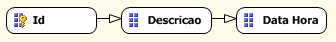
\includegraphics[scale=1]{images/A_DIM_Experimento.PNG}
%         \caption{Hierarquia da dimensão DIM\_Experimento}
%         \label{fig:ModeloOLAP}
% \end{figure}

\begin{itemize}
	\item
		\textbf{Tabela:} DIM\_Modelo\_Dinamico \\
		\textbf{Tipo:} Dimensional. \\
		\textbf{Descrição:} Representa qual dinâmica utilizada no experimento. \\
\end{itemize}
\begin{table}[!htbp]
	\caption{Dimensão DIM\_Modelo\_Dinamico}
	\centering
	\begin{tabular}{@{}llll@{}}
	\toprule
	\textbf{Nome} 	& \textbf{Tipo} & \textbf{PK} & \textbf{Descrição}           			\\ \midrule
	Id            	& INT           & x           & Identificador da dimensão modelo dinamico   \\
	Descricao     	& TEXT       &             & Descrição da dinamica utilizada        \\ \bottomrule
	\end{tabular}
\end{table}

% \begin{figure}[h]
%         \center
%         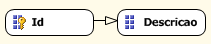
\includegraphics[scale=1]{images/A_DIM_Modelo_Dinamico.PNG}
%         \caption{Hierarquia da dimensão DIM\_Modelo\_Dinamico}
%         \label{fig:ModeloOLAP}
% \end{figure}

\begin{itemize}
	\item
		\textbf{Tabelas:} DIM\_R1 a DIM\_R10 \\
		\textbf{Tipo:} Dimensional. \\
		\textbf{Descrição:} Representa um dos dez principais resíduos para o experimento. \\
\end{itemize}
\begin{table}[!htbp]
	\caption{Dimensões DIM\_R1 a DIM\_R10}
	\centering
	\begin{tabular}{@{}llll@{}}
	\toprule
	\textbf{Nome} 	& \textbf{Tipo} & \textbf{PK} & \textbf{Descrição}           		\\ \midrule
	Id            	& INT           & x           & Identificador da dimensão residuo   \\
	Nome 		  & TEXT       &             & Nome do residuo 					   	\\ 
	Tipo          & TEXT       &             & Tipo do residuo           	   		\\ \bottomrule   
	\end{tabular}
\end{table}
	
\newpage

A Figura \ref{fig:hierarGrupoLiganteExperimentoModelo} apresenta a composição das hierarquias para as dimensões DIM\_Grupo, DIM\_Experimento, DIM\_Ligante e DIM\_Modelo\_Dinamico respectivamente. Já a Figura \ref{fig:HierarR1ateR10} apresenta a hierarquia para as dimensões dos resíduos de 1 à 10.

\begin{figure}[h]
        \center
        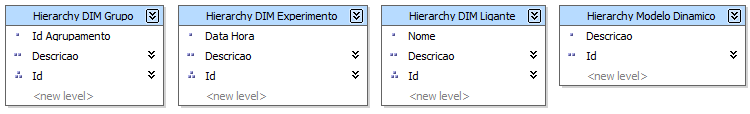
\includegraphics[scale=0.6]{images/Hierar_Grupo_Ligante_Experimento_Modelo.png}
        \caption{Hierarquias das dimensões Grupo, Ligante, Experimento e Modelo Dinâmico}
        \label{fig:hierarGrupoLiganteExperimentoModelo}
\end{figure}

\begin{figure}[h]
        \center
        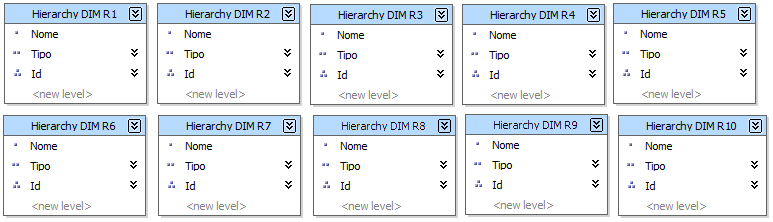
\includegraphics[scale=0.6]{images/Hierar_DIMR1_ate_10.png}
        \caption{Hierarquia das dimensões R1, R2, R3, R4, R5, R6, R7, R8, R9 e R10}
        \label{fig:HierarR1ateR10}
\end{figure}	

\section{Carga de dados no Analysis Services}
\label{sec:CargaDeDadosNoAnalysisServices}

Para o processo de carga dos dados foram desenvolvidos dois scripts e consiste na execução de ambos. O primeiro deles nomeado como ``criaDadosDIMTempo'' tem como objetivo fornecer um \emph{script} SQL para inserção dos dados para a dimensão tempo. O \emph{script} ``criaDadosDIMTempo'' recebe apenas um parâmetro de entrada para execução que é o número de picosegundos que vão ser populados na tabela do banco de dados. A saída é um comando de \emph{INSERT} do SQL para gravação na base de dados. O Algoritmo \ref{alg:criaDadosDIMTempo} descreve o funcionamento do \emph{script} ``criaDadosDIMTempo''. 

\floatname{algorithm}{Algoritmo}
\begin{algorithm}[H]
\caption{Algoritmo para popular os dados na dimensão tempo}
\label{alg:criaDadosDIMTempo}
{\fontsize{10}{10}\selectfont
\begin{algorithmic}[1]
	\STATE Seja P um valor inteiro maior que 1
	\STATE Seja L uma lista de valores
	\STATE Seja c um contador
	\FOR{iteração em P}
		\STATE Incrementa mais um em c
		\IF{c igual a 1000}
			\STATE Armazena o valor de P em L
			\STATE Grave o comando de inserção baseado em L
			\STATE Esvazie L
			\STATE Atribua zero em c
		\ELSE
			\STATE Armazena valor de P em L
		\ENDIF
	\ENDFOR
	\IF{L não estiver vazia}
		\STATE Grave o comando de inserção baseado em L
	\ENDIF
\end{algorithmic}
}
\end{algorithm}

O segundo \emph{script} desenvolvido, nomeado de ``criaDados'' é responsável por extrair e realizar a carga de todo o restante das informações contidas no \emph{data set} para a base de dados. Para sua execução são necessários 8 parâmetros de entrada, sendo 4 deles referentes às dimensões que serão populadas, e os outros 4 são arquivos distintos gerados pelos scripts executados previamente.

Os parâmetros de entrada para execução do script ``criaDados'' são os seguintes:
\begin{enumerate}
	\item CSV de entrada contendo os campos da dimensão DIM\_Grupo;
	\item CSV de entrada contendo os campos da dimensão DIM\_Ligante;
	\item CSV de entrada contendo os campos da dimensão DIM\_Experimento;
	\item CSV de entrada contendo os campos da dimensão DIM\_Modelo\_Dinamico;
	\item Arquivo de entrada contendo a lista dos resíduos relevantes;
	\item Arquivo de entrada contendo a relação de contatos por resíduo (gerado pelo Algoritmo \ref{alg:CalculoDistancia});
	\item Arquivo de entrada com dados de docagem (\emph{data set});
	\item Arquivo de entrada com o agrupamento das conformações;
\end{enumerate}

Por fim, após a execução completa do \emph{script}, é gerado os comandos de \emph{INSERT} em SQL para popular as informações no banco de dados. O Algoritmo \ref{alg:criaDadosFato} descreve o funcionamento do \emph{script} ``criaDados''.

\floatname{algorithm}{Algoritmo}
\begin{algorithm}[H]
\caption{Algoritmo para popular os dados na fato}
\label{alg:criaDadosFato}
{\fontsize{10}{10}\selectfont
\begin{algorithmic}[1]
	\STATE Seja L uma lista de ligantes
	\STATE Seja l um ligante em L
	\STATE Seja G uma lista de grupos
	\STATE Seja g um grupo em G
	\STATE Seja M uma lista de modelos dinâmicos
	\STATE Seja m um modelo dinâmico em M
	\STATE Seja E uma lista de experimentos
	\STATE Seja e um experimento em E
	\STATE Seja R uma lista de resíduos mais importantes
	\STATE Seja r um resíduo em R
	\STATE Seja S uma lista de numero de contato dos resíduos
	\STATE Seja s o numero de um contato em S
	\STATE Seja D a base de dados dos resultados da simulação de docagem molecular
	\STATE Seja d uma conformação em D
	\STATE Seja a um agrupamento de d
	\STATE Seja C uma lista de comandos para inserção
	\FOR{cada l em L}
		\STATE Grave o comando de inserção baseado em l
	\ENDFOR
        \FOR{cada g em G}
		\STATE Grave o comando de inserção baseado em g
        \ENDFOR
        \FOR{cada m em M}
		\STATE Grave o comando de inserção baseado em m
        \ENDFOR
        \FOR{cada e em E}
		\STATE Grave o comando de inserção baseado em e
        \ENDFOR
	\FOR{cada r em R}
		\STATE Grave o comando de inserção baseado em r
	\ENDFOR
	\FOR{cada d em D}
		\STATE Grave a em C
		\FOR{cada l em L}
			\FOR{cada s em S}
				\STATE Gravar o valor de s em C para a composição baseando em d, l e r
			\ENDFOR
			\IF{FEB de d for positiva}
				\STATE Gravar 0 para FEB de d em C
			\ELSE
				\STATE Gravar FEB de d em C
			\ENDIF
			\STATE Gravar RMSD de d em C
			\STATE Gravar o comando de inserção baseado em C
		\ENDFOR
	\ENDFOR
\end{algorithmic}
}
\end{algorithm}

Em suma, os scripts desenvolvidos para auxiliar no processo de ETL utilizados durante este trabalho foram executados na seguinte sequência:
\begin{enumerate}
    \item Execução do \emph{script} ``ajustaColunasDocking'' - Separar o resíduo NAH e cria um \emph{data set} auxiliar.
    \item Execução do \emph{script} ``calculaDistancia'' - Calcular distância Euclidiana par os dois \emph{data sets}.
    \item Execução do \emph{script} ``criaDadosDIMTempo'' - Popular a dimensão tempo no banco de dados.
    \item Execução do \emph{script} ``criaDados'' - Popular o restante das informações no banco de dados.
\end{enumerate}


